\index{error analysis}
\chapter{Error Analysis}
\newthought{Some call it Error. I call it Character.}

% ==============================================================================================
% INTRODUCTION BLOCK - 15 minutes

\section{The Why}


\index{conditioning}
\index{stability}
\index{consistency}
\index{convergence}
\newthought{Conditioning, Stability, Consistency and Convergence.} are fundamental concepts in numerical analysis that help us understand the behavior of numerical algorithms and their reliability in solving mathematical problems.
\index{model error}
\marginnote{\newthought{One last word on model error.} With $f(\cdot)$ we imply the exact model of a system. 
In practice, models are simplifications of reality, for a distance between two points A and B we might 
use a simplified Manhattan or Euclidean model that does not account for terrain, mode of travel, or obstacles. So keep in mind that our $f(\cdot)$ here, is another $\tilde{f}(\cdot)$.}


\newthought{Understanding Concepts} to describe the behavior and characteristics of numerical methods, let us:
\begin{itemize}
    \item Assess the sensitivity to small changes in the input data.
    \item Evaluate the sensitivity of the numerical solution to the small changes in the input data.
    \item Ensure that numerical methods produce accurate and reproducible results.
    \item Guarantee that our approximations converge to the true solution.
\end{itemize} 


\newthought{In machine learning and artificial intelligence,} especially when training large models on vast datasets, understanding these concepts is crucial.
Latest now, it should have become clear to you that training neural networks and other models, involves solving large-scale optimization problems, often requiring iterative numerical methods.
In Deep Learning convergence has the center stage, then almost as an afterthought comes Complexity - the number of operations and amount of time it takes to get there.

\marginnote{\newthought{Deep Learning by Goodfellow}, does a great job kick-starting you into numerical computation (Ch. 4) for machine learning. Check it out for further reading: \cite{DeepLearningBookNumericalComputation}.}

In general you will be able to later on evaluate and describe the characteristics of AI models $\theta$ with exactly these concepts.
So the maths aside, this will come in handy.






\newpage
\subsection{Hands On Experience}


For starters let's get an intuitive feel for these concepts with some simple examples.
Each concept will be illustrated with two quick exercises you can do by hand or in your head. 
It is two excercises as we want to highlight two sides of the same coin for each concept, introducing somewhat extremes on the spectrum.
Because you already know it, let's revisit our discretized sine function example from Chapter 1.




\newthought{Conditioning} is about how sensitive the solution is to small changes in the input data.

\begin{figure}[h]
    \centering
    % Requires: \usepackage{pgfplots}
    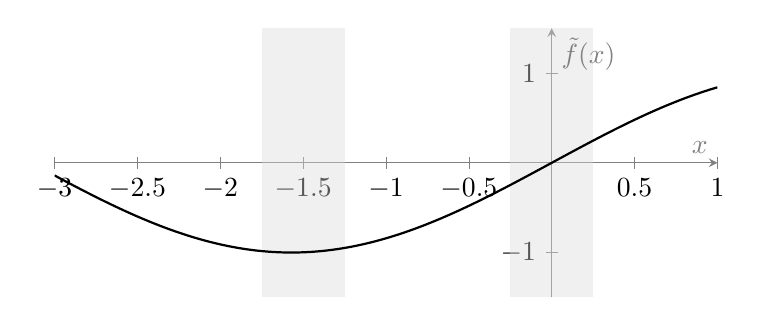
\begin{tikzpicture}
        \begin{axis}[
              width=10cm,
              height=5cm,
              axis x line=middle,
              axis y line=middle,
              xlabel={$x$},
              ylabel={$\tilde{f}(x)$},
              domain=-3:1,
              samples=100,
              ymin=-1.5, ymax=1.5,
              xmin=-3, xmax=1,
              legend style={at={(0.5,-0.2)},anchor=north},
              tick style={gray},
              label style={gray},
              axis line style={gray},
        ]
        % Transparent gray vertical band at x = -1.5, width = 0.5
        \addplot [
            draw=none, 
            fill=gray!30,
            fill opacity=0.4
        ] coordinates {(-1.75,-1.5) (-1.75,1.5) (-1.25,1.5) (-1.25,-1.5)};
        % Transparent gray vertical band at x = 0, width = 0.5
        \addplot [
            draw=none, 
            fill=gray!30,
            fill opacity=0.4
        ] coordinates {(-0.25,-1.5) (-0.25,1.5) (0.25,1.5) (0.25,-1.5)};
        % Continuous curve
        \addplot[black, thick, smooth] {sin(deg(x))};
        \end{axis}
    \end{tikzpicture}
    \caption{Continuous curve $\tilde{f}(x) = \sin(x)$ on $[-3,1]$ with two highlighted transparent vertical bands at $x=-1.5$ and $x=0$ (width $0.5$).}
    \label{fig:conditioning_bands}
\end{figure}

Let's assume for a moment that our approximated function equals the true function of the sine curve, however $\tilde{x}$ is a slightly perturbed version of $x$ due to measurement errors or rounding ($\pm 0.25$).
Now, look at the two gray bands at $x=-1.5$ and $x=0$. The first is a well-conditioned region, where small changes in $x$ lead to small changes in $f(x)$.
The second band around $x=0$ is ill-conditioned, where small changes in $x$ can lead to large relative changes in $f(x)$.

\index{floating-point representation}
\marginnote{\newthought{This is about floating-point representation} and not about step size or optimal approximation. Make sure to wrap your head around that, before moving on.}

\newthought{Stability} refers to the sensitivity of the numerical solution to the small changes in the input data.
\begin{figure}[h]
    \centering
    % Requires: \usepackage{pgfplots}
    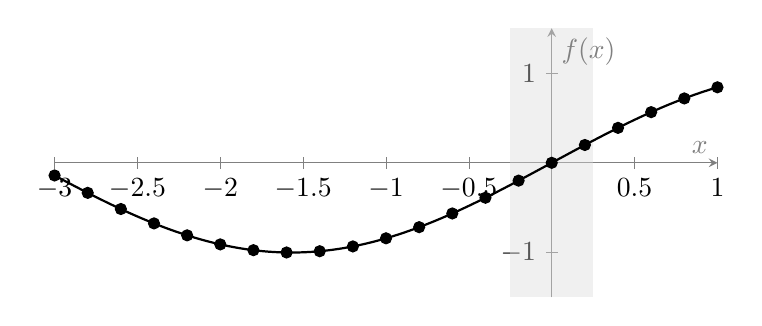
\begin{tikzpicture}
        \begin{axis}[
              width=10cm,
              height=5cm,
              axis x line=middle,
              axis y line=middle,
              xlabel={$x$},
              ylabel={$f(x)$},
              domain=-3:1,
              samples=100,
              ymin=-1.5, ymax=1.5,
              xmin=-3, xmax=1,
              legend style={at={(0.5,-0.2)},anchor=north},
              tick style={gray},
              label style={gray},
              axis line style={gray},
        ]
        % Transparent gray vertical band at x = 0, width = 0.5
        \addplot [
            draw=none, 
            fill=gray!30,
            fill opacity=0.4
        ] coordinates {(-0.25,-1.5) (-0.25,1.5) (0.25,1.5) (0.25,-1.5)};
        % Continuous curve
        \addplot[black, thick, smooth] {sin(deg(x))};
        % Discretized points for h=0.2
        \addplot[black, only marks, mark=*] coordinates {
            (-3.0, -0.1411)
            (-2.8, -0.33499)
            (-2.6, -0.51504)
            (-2.4, -0.67546)
            (-2.2, -0.80850)
            (-2.0, -0.90930)
            (-1.8, -0.97385)
            (-1.6, -0.99957)
            (-1.4, -0.98545)
            (-1.2, -0.93204)
            (-1.0, -0.84147)
            (-0.8, -0.71736)
            (-0.6, -0.56464)
            (-0.4, -0.38942)
            (-0.2, -0.19867)
            (0.0, 0.0)
            (0.2, 0.19867)
            (0.4, 0.38942)
            (0.6, 0.56464)
            (0.8, 0.71736)
            (1.0, 0.84147)
        };
        \end{axis}
    \end{tikzpicture}
    \caption{Continuous curve $f(x)_{.2} = \sin(x)$ on $[-3,1]$ with a highlighted transparent vertical band at $x=0$ (width $0.5$), and discretized points with step size $h=0.2$.}
    \label{fig:stability_h02}
\end{figure}

\begin{figure}[h]
    \centering
    % Requires: \usepackage{pgfplots}
    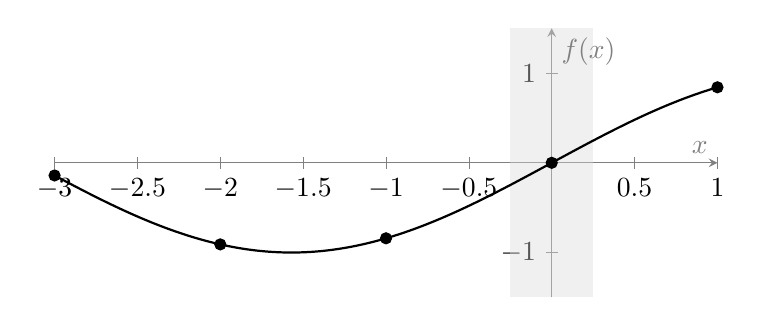
\begin{tikzpicture}
        \begin{axis}[
              width=10cm,
              height=5cm,
              axis x line=middle,
              axis y line=middle,
              xlabel={$x$},
              ylabel={$f(x)$},
              domain=-3:1,
              samples=100,
              ymin=-1.5, ymax=1.5,
              xmin=-3, xmax=1,
              legend style={at={(0.5,-0.2)},anchor=north},
              tick style={gray},
              label style={gray},
              axis line style={gray},
        ]
        % Transparent gray vertical band at x = 0, width = 0.5
        \addplot [
            draw=none, 
            fill=gray!30,
            fill opacity=0.4
        ] coordinates {(-0.25,-1.5) (-0.25,1.5) (0.25,1.5) (0.25,-1.5)};
        % Continuous curve
        \addplot[black, thick, smooth] {sin(deg(x))};
        % Discretized points for h=1
        \addplot[black, only marks, mark=*] coordinates {
            (-3, -0.1411)
            (-2, -0.9093)
            (-1, -0.8415)
            (0, 0)
            (1, 0.8415)
        };
        \end{axis}
    \end{tikzpicture}
    \caption{Continuous curve $f(x)_{1.} = \sin(x)$ on $[-3,1]$ with a highlighted transparent vertical band at $x=0$ (width $0.5$), and discretized points with step size $h=1$.}
    \label{fig:stability_h1}
\end{figure}

When paying attention to the gray band around $x=0$, we can see that in the first figure with step size $h=0.2$, 
the discretized points closely follow the sine curve, indicating a instability due to the changes in $\tilde{x} \pm 0.25$, resulting in fluctuations
in the computed values of $\tilde{f}(\tilde{x})$.
In contrast, the second figure with step size $h=1$ shows only a single discretized point within the gray band, 
leading to a stable approximation of the sine curve in that region - regardless of the deviations in $\tilde{x}$.


\newthought{Consistency} quantifies how well our numerical method matches the exact solution of the original problem. 
To make it easy to follow, we introduce a discretization with a step size of $h=1$ and one with a step size of $h=0.2$.

\begin{figure}[h]
    \centering
    % Requires: \usepackage{pgfplots}
    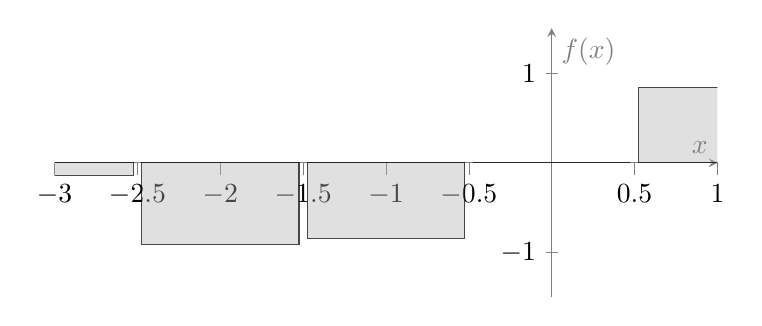
\begin{tikzpicture}
        \begin{axis}[
              width=10cm,
              height=5cm,
              axis x line=middle,
              axis y line=middle,
              xlabel={$x$},
              ylabel={$f(x)$},
              domain=-3:1,
              samples=100,
              ymin=-1.5, ymax=1.5,
              xmin=-3, xmax=1,
              legend style={at={(0.5,-0.2)},anchor=north},
              tick style={gray},
              label style={gray},
              axis line style={gray},
              ybar,
              bar width=0.95,
        ]
        % Bar plot for discretized points with h=1 (semi-transparent)
        \addplot[black, fill=gray!60, fill opacity=0.4, draw opacity=0.7] coordinates {
            (-3, -0.1411)
            (-2, -0.9093)
            (-1, -0.8415)
            (0, 0)
            (1, 0.8415)
        };
        \end{axis}
    \end{tikzpicture}
    \caption{Bar plot of discretized values $f(x)_{1.} = \sin(x)$ on $[-3,1]$ with step size $h=1$.}
    \label{fig:consistency_h1}
\end{figure}

\begin{figure}[h]
    \centering
    % Requires: \usepackage{pgfplots}
    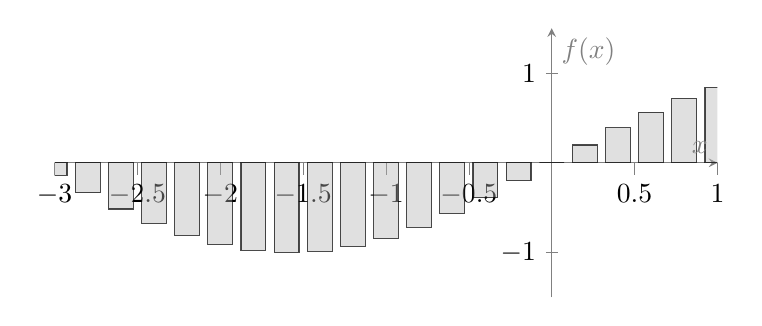
\begin{tikzpicture}
        \begin{axis}[
              width=10cm,
              height=5cm,
              axis x line=middle,
              axis y line=middle,
              xlabel={$x$},
              ylabel={$f(x)$},
              domain=-3:1,
              samples=100,
              ymin=-1.5, ymax=1.5,
              xmin=-3, xmax=1,
              legend style={at={(0.5,-0.2)},anchor=north},
              tick style={gray},
              label style={gray},
              axis line style={gray},
              ybar,
              bar width=0.15,
        ]
        % Bar plot for discretized points with h=0.2 (semi-transparent)
        \addplot[black, fill=gray!60, fill opacity=0.4, draw opacity=0.7] coordinates {
            (-3.0, -0.1411)
            (-2.8, -0.33499)
            (-2.6, -0.51504)
            (-2.4, -0.67546)
            (-2.2, -0.80850)
            (-2.0, -0.90930)
            (-1.8, -0.97385)
            (-1.6, -0.99957)
            (-1.4, -0.98545)
            (-1.2, -0.93204)
            (-1.0, -0.84147)
            (-0.8, -0.71736)
            (-0.6, -0.56464)
            (-0.4, -0.38942)
            (-0.2, -0.19867)
            (0.0, 0.0)
            (0.2, 0.19867)
            (0.4, 0.38942)
            (0.6, 0.56464)
            (0.8, 0.71736)
            (1.0, 0.84147)
        };
        \end{axis}
    \end{tikzpicture}
    \caption{Bar plot of discretized values $f(x)_{.2} = \sin(x)$ on $[-3,1]$ with step size $h=0.2$.}
    \label{fig:consistency_h02}
\end{figure}

Again, it is easy to see that for infinitesimally small step sizes $h \to 0$, the discretized points will get closer and closer to the true sine curve.
In the end resulting in a perfect match between the numerical method and the exact solution of the original problem, which means optimal consistency.

\marginnote{\newthought{Intuitive convergence example with sine,} wanted. If you have a better idea to have the examples stick to the sine context, let me know.}


\newthought{Convergence} emerges when we combine the ideas of stability and consistency.
A numerical method is convergent if, as we refine our approximation $\tilde{f}(x)$ (for example, by decreasing the step size $h$), 
the computed solution approaches the exact solution of the problem regardless of the deviations in $\tilde{x}$, or by implicitly accounting for them.



\vspace{2.5em}
\newthought{The Learning Objectives} of this chapter aim at providing you with the abilities to:
\begin{itemize}
    \item Have an intuition about the concepts of conditioning, stability, consistency, and convergence in numerical methods.
    \item Analyze simple numerical problems quantitatively with respect to these concepts.
\end{itemize}



















\newpage




% ==============================================================================================
% MAIN THEORY BLOCK - 15 minutes

\newpage
\section{Quantitative Characterization of Numerical Methods}

\newthought{We introduce} the following notation, Let $f(\cdot)$ denote the exact (analytical) solution of a problem, 
and let $\tilde{f}(\cdot)$ represent the numerical method (algorithm) that provides an approximation. 
The variable $x$ stands for the exact input data, while $\tilde{x}$ refers to the actual input data used, 
which may be perturbed, for example, by measurement errors or rounding.

\newthought{Conditioning} describes how sensitive a problem's solution is to small changes in the input data. 
Formally, the conditioning of a problem at $x$ can be quantified by the condition number $\kappa$:

\begin{equation}
    \kappa = \left| f(x) - f(\tilde{x}) \right|.
\end{equation}


\newthought{$\kappa$} is often normalized to express it as a relative measure.




\newthought{Stability} is given if small errors in the input or intermediate steps do not result in disproportionately 
large errors in the output. 
Mathematically, a stable method ensures that the error in the computed solution $\tilde{f}(\tilde{x})$ remains bounded by a constant multiple of the error in the input data:

\begin{equation}
    \left| \tilde{f}(\tilde{x}) - \tilde{f}(x) \right| \leq s \cdot \left| \tilde{x} - x \right|,
\end{equation}

where $s$ is a constant. For $s \approx 1$, the error in the 
computed solution develops linearly with the error in the input data.




\newthought{Consistency} means how well our numerical solution approximates the exact solution of the original problem:
\begin{equation}
    \left| \tilde{f}(x) - f(x) \right| \leq c
\end{equation}
where $c$ is a constant that quantifies the consistency error.




\marginnote{\newthought{Convergence} usually aims for zero error margin, which is often the exact solution $f(x)$. However, often we will experience non-zero convergence.
If the method converges to a value different from $f(x)$, this indicates a systematic error (bias) in the method.}


\newthought{Convergence} in general refers to our approximation reaching a specific stable limit.
A method is convergent if:
\begin{equation}
   \left| \tilde{f}(\tilde{x}) - f(x) \right| \to \lim
\end{equation}
That is, as both the real solution is approximated and deviations in data are controlled by an error margin.











% ==============================================================================================
% STUDENT ACTIVATION BLOCK - 15 minutes


\newpage
\section{Examples \& Excercises}


\newthought{Finding the Minimum} of the sine function on the interval $[-3, 1]$ one more time. 
Again discretize the function with two different step sizes $h=1$ and $h=0.2$. Further assume that the input 
data $x$ is perturbed by $\tilde{x} = x \pm 0.25$ due to measurement errors and has a precision of two decimal places.
Now analyze the conditioning, stability, consistency, and convergence of the numerical method used 
to find the minimum in both cases. Quantify the characteristics using the formulas provided in the previous section.


\newthought{Conditioning} is independent of the numerical method used, as it describes the sensitivity of the problem itself to changes in input data.
Thus, the conditioning can be analyzed by purely examining how small changes in $x$ affect the value of $\sin(x)$. 
We can see that around $x=-1$, where the minimum is, the sine function is relatively flat, indicating good conditioning. For sake of comparison we also consider
$x=0$, where the sine function changes rapidly, indicating poor conditioning. Solving this on paper we focus on these 
two regions to quantify the conditioning.


% Quantitative analysis of conditioning at two regions: x = -1 (well-conditioned) and x = 0 (ill-conditioned)
\begin{align*}
    \kappa(-1, +0.25) &= |\sin(-1) - \sin(-0.75)| \\
    &\approx |{-0.8415} - ({-0.6816})| \\
    &= 0.1599 \\[1em]   
    \kappa(-1, -0.25) &= |\sin(-1) - \sin(-1.25)| \\
    &\approx |{-0.8415} - ({-0.9489})| \\
    &= 0.1074 \\[1em]
\end{align*}
Which shows well-conditioning with $0.1074 \leq \kappa \leq 0.1599$.


\begin{align*}
    \kappa(0, +0.25) &= |\sin(0) - \sin(0.25)|\\
    &\approx |0 - 0.2474| \\
    &= 0.2474 \\[1em]
    \kappa(0, -0.25) &= |\sin(0) - \sin(-0.25)| \\
    &\approx |0 - (-0.2474)| \\
    &= 0.2474 \\
\end{align*}
Which shows ill-conditioning with $\kappa \leq 0.247$.




\newthought{Stability} depends on the numerical method used to approximate the sine function and find its minimum.
For the discretization with step size $h=1$, the method is stable as small changes in $\tilde{x}$ lead to small changes in the computed values of $\tilde{f}(\tilde{x})$.
For the discretization with step size $h=0.2$, the method is less stable, as small changes in $\tilde{x}$ can lead to larger fluctuations in the computed values of $\tilde{f}(\tilde{x})$.
Quantifying stability for both cases involves calculating the constant $s$ in the stability inequality:

\marginnote{\newthought{Stability,} equals the conditioning of the system, for $h \to 0$. Show it.}
% tilde f --> f

\begin{equation}
    \left| \tilde{f}(\tilde{x}) - \tilde{f}(x) \right| \leq s \cdot \left| \tilde{x} - x \right|
\end{equation}

Due to symmetry we only consider the case $\tilde{x} = x + 0.25$.
\marginnote{\newthought{a)} See how the step size $h=1$ leads to the same function value at both points. For reference, Fig.~\ref{fig:consistency_h1}}

\vspace{1em}
For $h=1$:
\begin{align*}
    s_{h=1, x=-1} \cdot |\tilde{x} - x| &= |\tilde{f}(\tilde{x}) - \tilde{f}(x)| \\
    &= |\tilde{f}_1(-0.75) - \tilde{f}_1(-1)|\\ 
    &= |\tilde{f}_1(-1) - \tilde{f}_1(-1)| \text{ see A)}\\ 
    s_{h=1, x=0} &\approx 0 \div 0.25 \\
    &\approx 0
\end{align*}

\vspace{1em}
For $h=0.2$:
\begin{align*}
    s_{h=0.2, x=-1} \cdot |\tilde{x} - x| &= |\tilde{f}(\tilde{x}) - \tilde{f}(x)| \\
    &= |\tilde{f}_{0.2}(-0.75) - \tilde{f}_{0.2}(-1)| \\
    &= |\tilde{f}_{0.2}(-0.8) - \tilde{f}_{0.2}(-1)| \\ 
    &= |-0.71736 - (-0.84147)| \\
    s_{h=0.2, x=-1}  &= 0.12411 \div 0.25 \\
    &\approx 0.4964
\end{align*}

Be aware that stability has anomalies in border regions of the discretization. This is especially a problem for piece-wise constant approximations.

\newthought{Consistency} is determined by comparing the numerical solution $\tilde{f}(x)$ with the exact solution $f(x)$ for the minimum of the sine function in $[-3,1]$.
To again quantify consistency for both step sizes, we calculate the constant $c$ in the consistency inequality:

\begin{equation}
    \left| \tilde{f}(x) - f(x) \right| \leq c
\end{equation}

\marginnote{\newthought{Remember} the analytical solution of min(sin(x)) on $[-3,1]$ - revisit Chapter 1.}

For $h=1$:
\begin{align*}
    c_1 &\geq \left| \tilde{f}_1(-\frac{\pi}{2}) - f(-\frac{\pi}{2}) \right| \\
    &\geq \left| \tilde{f}_{1}(-1) - f(-\frac{\pi}{2}) \right| \\
    &\geq \left| -0.84147 - (-1) \right| \\
    &\geq 0.15853
\end{align*}


For $h=0.2$:
\begin{align*}
    c_{0.2} &\geq \left| \tilde{f}_{0.2}(-\frac{\pi}{2}) - f(-\frac{\pi}{2}) \right| \\
    &\geq \left| \tilde{f}_{0.2}(-1.2) - f(-\frac{\pi}{2}) \right| \\
    &\geq \left| -0.94898 - (-1) \right| \\
    &\geq 0.05102
\end{align*}

Consistency improves with smaller step sizes, as expected.




\newthought{Convergence} combines the ideas of stability and consistency.
To quantify convergence we calculate the total error between the numerical solution $\tilde{f}(\tilde{x})$ and the exact solution $f(x)$:

\begin{equation}
    \left| \tilde{f}(\tilde{x}) - f(x) \right|.
\end{equation}

\vspace{1em}
Due to symmetry we only consider the case $\tilde{x} = x + 0.25$.

For $h=1$:
\begin{align*}
    \left| \tilde{f}_1(\tilde{x}) - f(x) \right| 
    \left| \tilde{f}_1(-1) - f(-\frac{\pi}{2}) \right| \\
    \left| \tilde{f}_1(-0.75) - f(-\frac{\pi}{2}) \right| \\
    \left| \tilde{f}_1(-1) - f(-\frac{\pi}{2}) \right| \\
    \left| -0.84147 - (-1) \right| \\
    = 0.1599
\end{align*}

\vspace{1em}
For $h=0.2$:
\begin{align*}
    \left| \tilde{f}_{0.2}(\tilde{x}) - f(x) \right| 
    \left| \tilde{f}_1(-1.2) - f(-\frac{\pi}{2}) \right| \\
    \left| \tilde{f}_{0.2}(-0.95) - f(-\frac{\pi}{2}) \right| \\
    \left| \tilde{f}_{0.2}(-1) - f(-\frac{\pi}{2}) \right| \\
    \left| -0.84147 - (-1) \right| \\
    = 0.1599
\end{align*}

\newthought{Due to} the stability issues in the $h=0.2$ case, convergence does not improve with smaller step sizes in this operation point.
This allows us to understand two things, both numerical solutions convergence to the same limit. 
Judging from these two results we could also say that the method of iteratively reducing the step size $h$ converges to the same limit as well.
Notice that we use the characteristics for both a numerical solution and the numerical method.


% CODE

\marginnote{\newthought{Code} is again to be found here \url{https://github.com/Quillstacks/lecturecode_numericalmethods.git}.}

\index{numerical solution}
\index{numerical method}
\newthought{Hands on compute-driven error analysis.} Let's brute-force our way through the error analysis of solving the two-equation system of Chapter 1.
You will determine and optimize the conditioning, stability, consistency, and convergence of the numerical solution by optimizing the numerical method.





\section{Self-Reflection and Recap}

%<Discussion about the findings and the learned concepts>
\index{self-reflection}
\newthought{Self-Reflection} Questions which can guide your thoughts during the excercises and afterwards:
\begin{itemize}
    \item Compared to the numerical solution to the minimum of the sine function, how well conditioned is the two-equation system? 
    \item Does stability converge with smaller step sizes in the two-equation system? Against what? 
    \item How do perturbations in the input data affect the numerical solution of the two-equation system? Is there an interplay with step size?
    \item Compare convergence with stability and consistency. What do you observe? Can you express your observations in terms of bias and variance?
    \item For ever smaller step sizes, do you observe a limit to the accuracy of the numerical solution? If so, why?
    \item What is another problem you observe while refining the step size? 
\end{itemize}

%<Recap of Key Concepts>
\index{key concepts}
\newthought{Recap} of Key Concepts:
\begin{itemize}
    \item Conditiioning, Stability, Consistency, and Convergence are fundamental concepts in numerical analysis that help us understand the behavior of numerical algorithms.
    \item These concepts can be expressed qualitatively and quantitatively to analyze numerical solutions and methods.
\end{itemize}



\index{brute-force method}
\marginnote{\newthought{Teaser.} So far we did brute-force numerical solutions. Can you think of a way to refine brute-force methods 
to get better results with less effort? Use the code of this lecture to design and test your idea.}

\index{numerical algorithms}
\newthought{Now that we} understand and can characterize the behavior of individual numerical solutions, 
we can move on to understanding how to analyze entire numerical methods and algorithms. So far we have taken the assumption of where to look for a solution, inside a specific interval, for granted.
This is usually not a given, and we will need to move away from local optimization methods in the next lecture. 




%%%%%%%%%%%%%%%%%%%%%%%%%%%%%%%%%%%%%%%%%%%%%%%%%%%%%%%%%%%%%%%%%%%%%%%%%%%%%%
